\documentclass[11pt, twocolumn, a4paper]{article}

\usepackage{graphicx}
\setlength{\oddsidemargin}{0.0 cm}
\setlength{\evensidemargin}{0.0 cm}
\setlength{\topmargin}{-1cm}
\setlength{\textheight}{24 cm}
\setlength{\textwidth}{16 cm}

\newcommand{\ttbarm}{\mathrm{t \overline{t} \; }}
\newcommand{\ttbar}{$\mathrm{t \overline{t} \; }$}

\pagestyle{plain}

\setlength{\parindent}{0in}

\usepackage[
  locale=DE,
  separate-uncertainty=true,
  decimalsymbol=.,
  per-mode=symbol-or-fraction,
]{siunitx}
\usepackage{amsmath,amssymb}

\begin{document}
\thispagestyle{empty}

\author{Salvatore La Cagnina}

\title{Summary of `OPAL Collaboration, {\it 'A search for the top and $b'$ quarks in hadronic $Z^0$ decays'}}

\maketitle

%####################################################################################################################
%###################################################EINLEITUNG#######################################################
%####################################################################################################################
In the paper a search for the top and new heavy $b'$ is presented.
The search has been performed by the OPAL collaboration with data from $e^+ e^-$ collision provided by LEP at CERN and collected with a center of mass energy of $\SI{91.26}{GeV}$.
The data set corresponds to an integrated luminosity of ${\;\mathcal{L}=\SI{72.4}{nb^{-1}}}$.
Since the new quarks are searched in hadronic $Z^0$ decays the center of mass energy is chosen near the $Z^0$ pole mass in order to produce $Z^0$ bosons due to resonance.\\
%####################################################################################################################
%###################################################MOTIVATION#######################################################
%####################################################################################################################
The Standard Model provides evidence towards the existence of the top quark, which has not been found by the time the search has been performed, due to the bottom quark as its isospin doublet partner missing neutral current decays and showing a forward-backward charge asymmetry in $e^+ e^-$ annihilation experiments.
An additional fermion family with a possible $b'$ quark has no constrain towards its mass due to the missing Standard Model prediction.
Therefore, a $b'$ could be lighter then a top quark.
%This additional quark can either decay in a charged current ${b' \rightarrow c W}$ including a small mixing element ${V_{cb'}}$, in neutral current ${b' \rightarrow b\gamma}$,${b' \rightarrow bg}$ or including the possibility of a light charged Higgs doublet the top and $b'$ could decay through the channels ${t \rightarrow bH^+}$ and ${b' \rightarrow cH^-}$.\\
This additional quark can either decay in a charged current,neutral current or through a light charged Higgs doublet expanding the scalar sector of the Standard Model.\\
%####################################################################################################################
%###################################################DETEKTOR#########################################################
%####################################################################################################################
The main components of the detector relevant for the analysis are the central tracking chamber and the electromagnetic calorimeter (ECAL).
In addition,the time-of-flight scintillation counter array is used in order to identify particles originating from the interaction point by timing their appearance with the collision time.
The tracking chamber is used to track charged particles like those found in hadronic jets.
It is located inside a magnet solenoid and covers $\SI{94}{\%}$ of the $4\pi$ plane.
The ECAL uses cylindrically aligned lead glass blocks and endcap arrays covering $\SI{98}{\%}$ of the $4\pi$ plane.\\
%It covers an angular range of ${|\cos{(\theta)}|\le \num{0.92}}$ and is located inside a magnet solenoid.
%The electromagnetic calorimeter uses cylindrically aligned lead glass blocks covering ${|\cos{(\theta)}|\le \num{0.82}}$ and endcap arrays covering $\num{0.81} \le {|\cos{(\theta)}|\le \num{0.98}}$.
%Most of the energy ($\SI{60}{\%}$) of multihadronic $Z^0$ events is absorbed in the ECAL.\\
%####################################################################################################################
%###################################################TIGGER EVENT SELECTION###########################################
%####################################################################################################################
The events are first selected using an online trigger in order to primarily distinguish between hadronic $Z^0$ events and background like tau pair production, two-photon processes, beam-pipe interaction and cosmic radiation.
This first selection criteria are an energy disposition exceeding ${\SI{6}{GeV}}$ in the ECAL, a signal in more then two non-adjacent scintillator caps in the time-of-flight counter array or the presence of at least two tracks with $p_T > {\SI{450}{MeV}}$ pointing towards the collision point.\\
%####################################################################################################################
%###################################################SHAPE VARIABLES##################################################
%####################################################################################################################
This analysis is based on the information provided by event shape variables.
Those event shape variables contain information about the topological form of an event and are sensitive to new heavy quarks due to the topological change of the decays with heavy patricles creating more perpendicular momentum.
One advantage for the use of shape variables for obtaining mass limits of the top quark toward other methods like high $p_T$ detection of semi leptonic quark decays, is the independence of Standard Model predictions for the branching ratios.
Due to inherent quark fragmentation the shape variables have a new source of uncertainties which, however, are reasonably well understood for the purpose of this search.
Those events shape variables are for example thrust, sphericity and acoplanarity.
For quark masses between $\SI{25}{GeV}$ and $\SI{45}{GeV}$ acoplanarity is the most effective variable which is defined as
\begin{equation*}
	A = 4 \, min\left(\frac{\sum_i |p_{i,T}|}{\sum_i |p_i|}\right)
\end{equation*}
where $p_{i,T}$ is the momentum of particle $i$ perpendicular to the plane containing most of the total momenta of all particles and is therefore the main focus of this search.
The contribution of the heavy quarks would lead to a higher value of acoplanarity in the events.
%####################################################################################################################
%###################################################EVENT SELECTION##################################################
%####################################################################################################################
In order to implement the event shape analysis further event selection criteria are implemented.
These are at least 8 separated energy clusters with more energy then $\SI{200}{MeV}$ in the barrel or $\SI{500}{MeV}$ in the endcap part of the ECAL, a sum of the energy clusters greater then $\SI{10}{GeV}$ and a range of the clusters within ${|\cos{(\theta)}|\le \num{0.96}}$. 
The selection for the tracking chamber consists of at least $20$ measured points in a track, $p_T > \SI{150}{MeV}$ a scalar sum of the track momenta greater then $\SI{10}{GeV}$ and the tracks have to lie within the range of ${|\cos{(\theta)}|\le \num{0.86}}$.\\
%####################################################################################################################
%###################################################DIE ANALYSE######################################################
%####################################################################################################################
The analysis for the search is performed in both the ECAL and the tracking chamber separately in order to yield a crosscheck and only uses charge current with a mass of $\SI{35}{GeV}$ for the Monte Carlo predictions which are provided for five quarks and five quarks + top or b'.
The resulting distribution of the acoplanarity for the ECAL and the mentioned Monte Carlo can be seen in fig. \ref{fig:aco}.
\begin{figure}
	\centering
	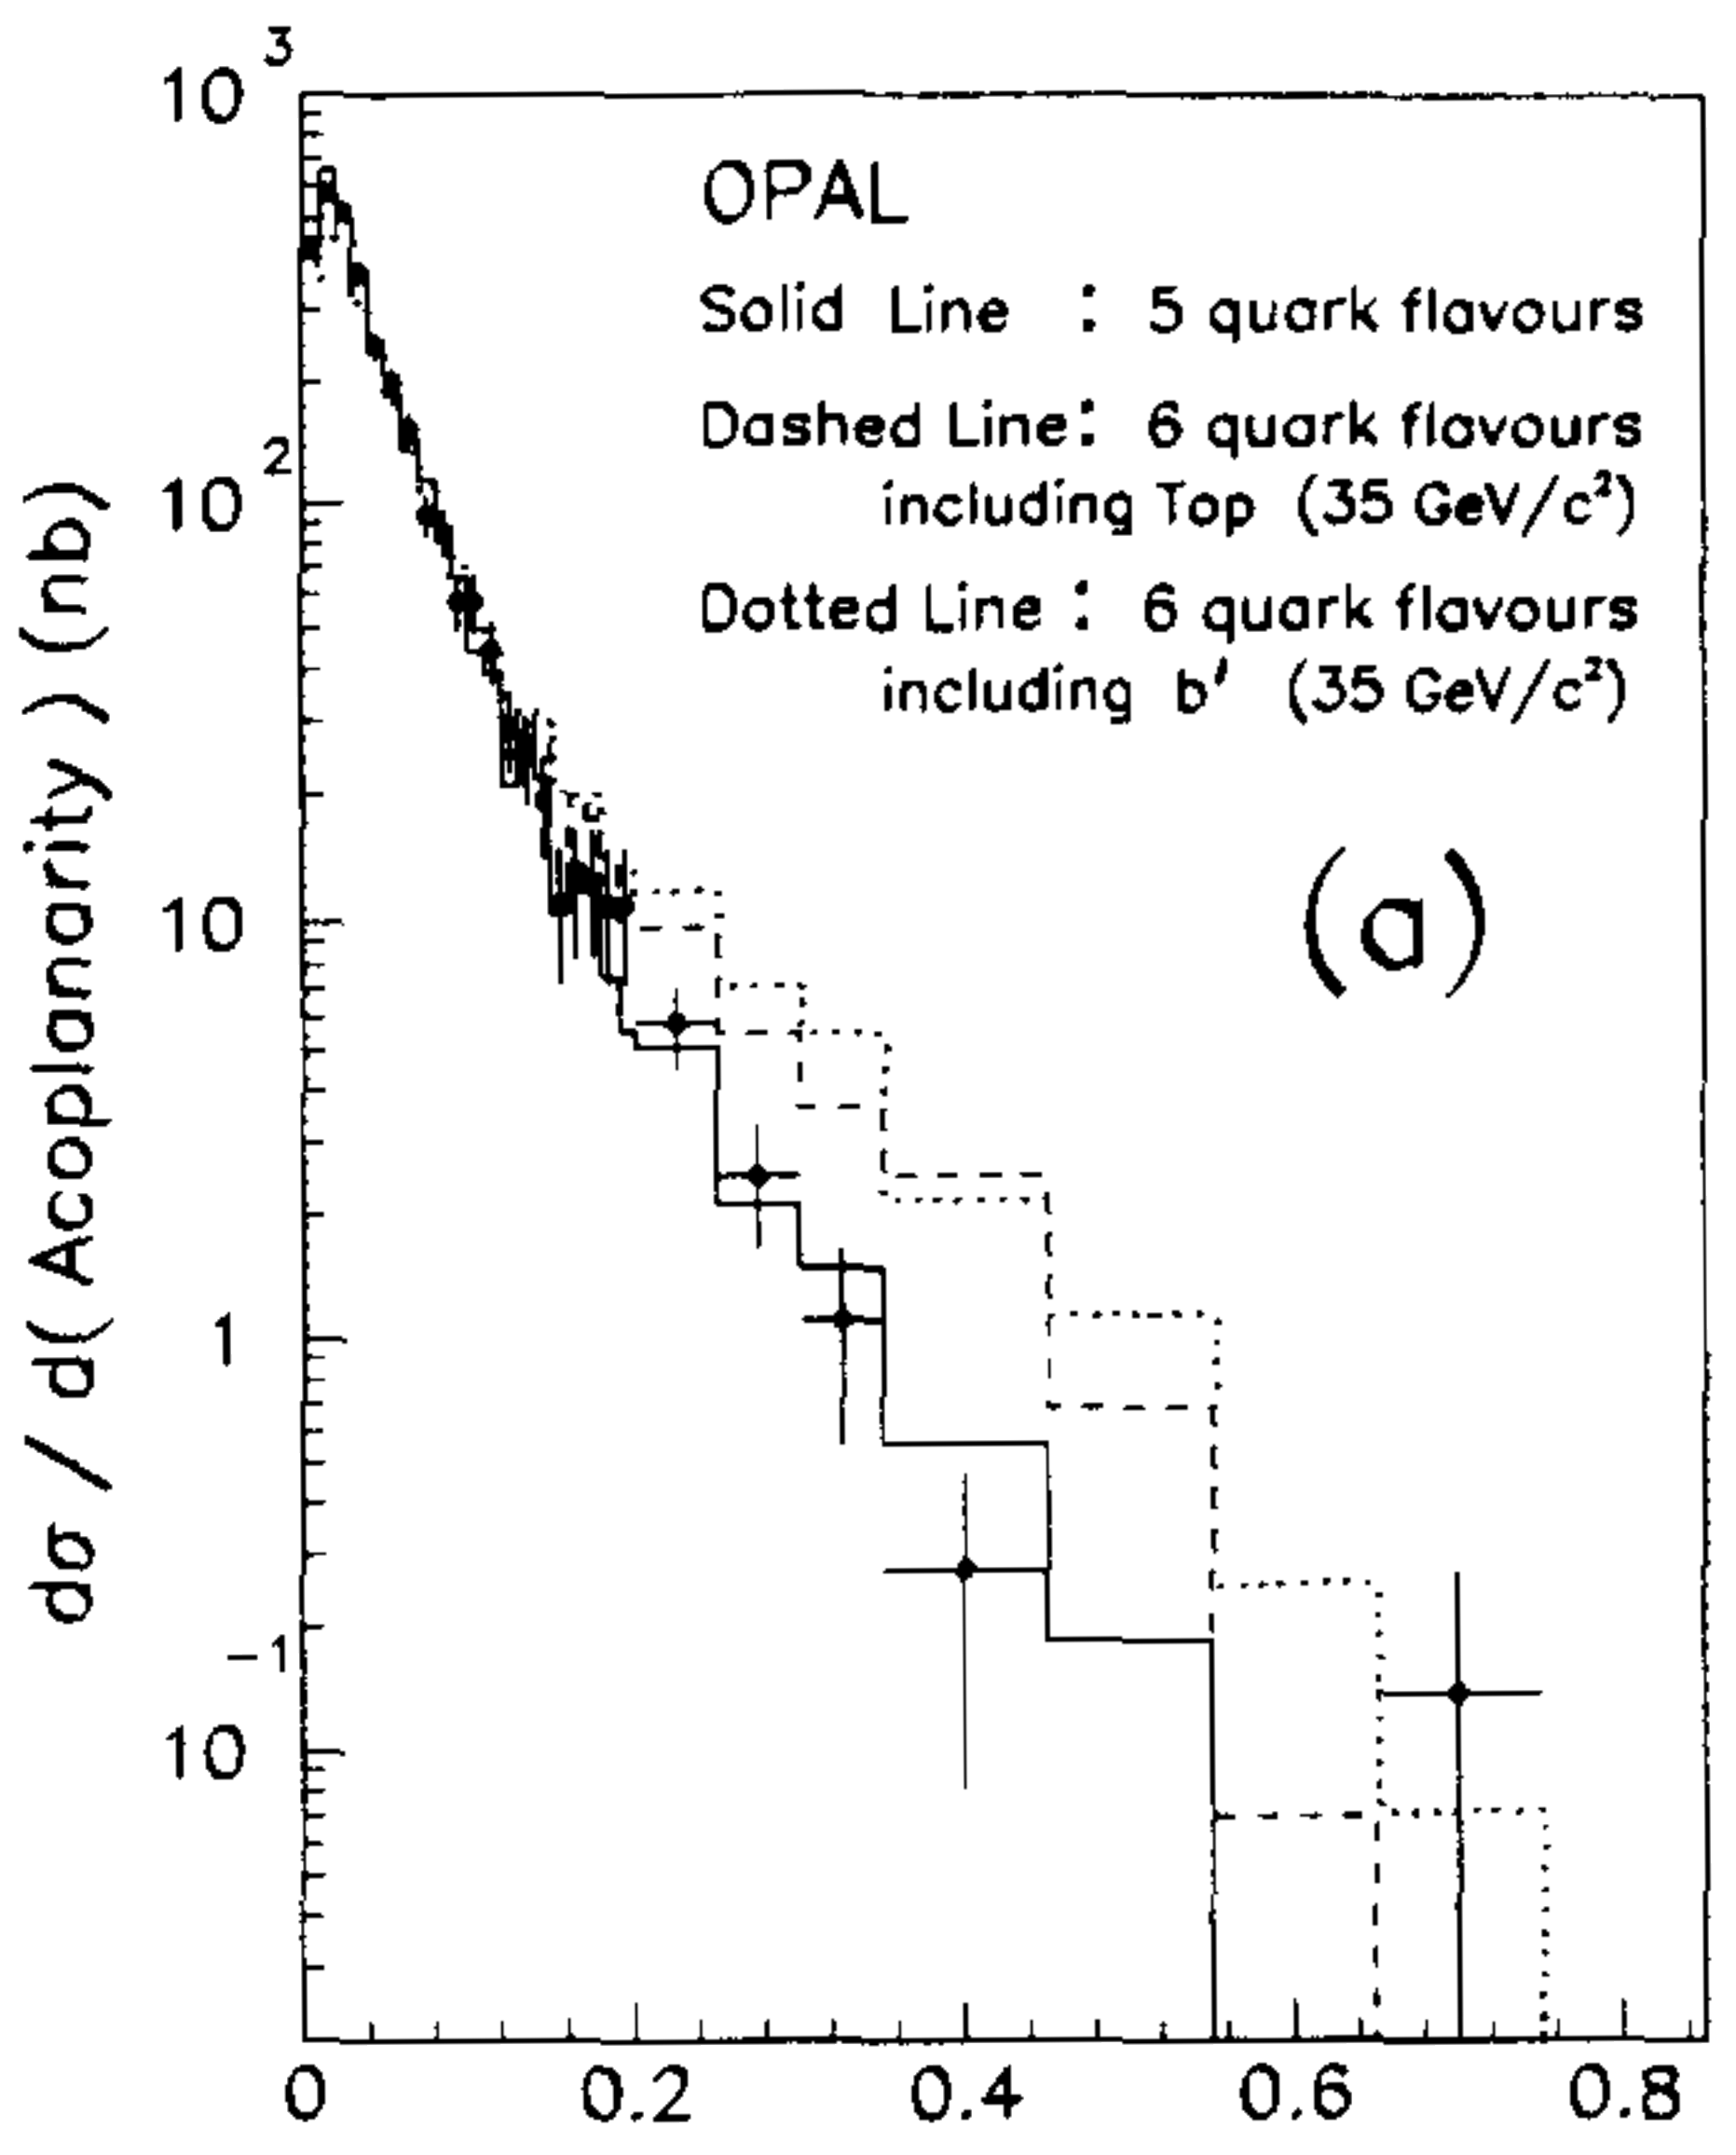
\includegraphics[width=0.5\textwidth]{plot.png}
	\caption{Acoplanarity measured by the electromagnetic calorimeter and Monte Carlo with charged current decays of top and $b'$ for a mass of $\SI{35}{GeV}$.\cite{paper}}
	\label{fig:aco}
\end{figure}
In the figure a good agreement between the data and the Monte Marlo using five quark is shown.
This result is supported by the data of the sphericity and thrust and also by the track chamber measurement yielding a cross check of the result.
Therefore there is no further evidence for a sixth quark within the kinematic limits of this analysis.\\
%####################################################################################################################
%###################################################MASSEN LIMITS####################################################
%####################################################################################################################
Even though this analysis does not provide evidence for a new heavy quark mass limits for these possible quarks can be derived.
The mass limits are calculated separately for the different decay modes of the heavy quarks.
For the calculation the following set of parameters have been used.
The masses ${m(Z^0)=\SI{91.01}{GeV}}$, ${m(H^0) = \SI{100}{GeV}}$ and the strong coupling constant ${\alpha_s=0.12}$.
For the decay of into the charged Higgs doublet the mass of the charged Higgs is set to $\SI{23}{GeV}$.
However, for this decay channel it is assumed that $H^\pm$ exclusively decays into $cs$ states.
Choosing the least stringent mass limit for both top and $b'$ of all calculated limits, the resulting limits at $\SI{95}{\%}$ confidence level are ${m(t) > \SI{44.5}{GeV}}$ ${m(b') > \SI{45.2}{GeV}}$.\\
%####################################################################################################################
%###################################################EINORDNUNG#######################################################
%####################################################################################################################
Considering the 


\begin{thebibliography}{99}
\bibitem{paper} OPAL Collaboration, A search for the top and $b'$ quarks in hadronic $Z^0$ decays, Phys. Lett. B 236 (1990) 364
\end{thebibliography}



\end{document}


%\begin{figure}[ht!]
%  \begin{center}
%    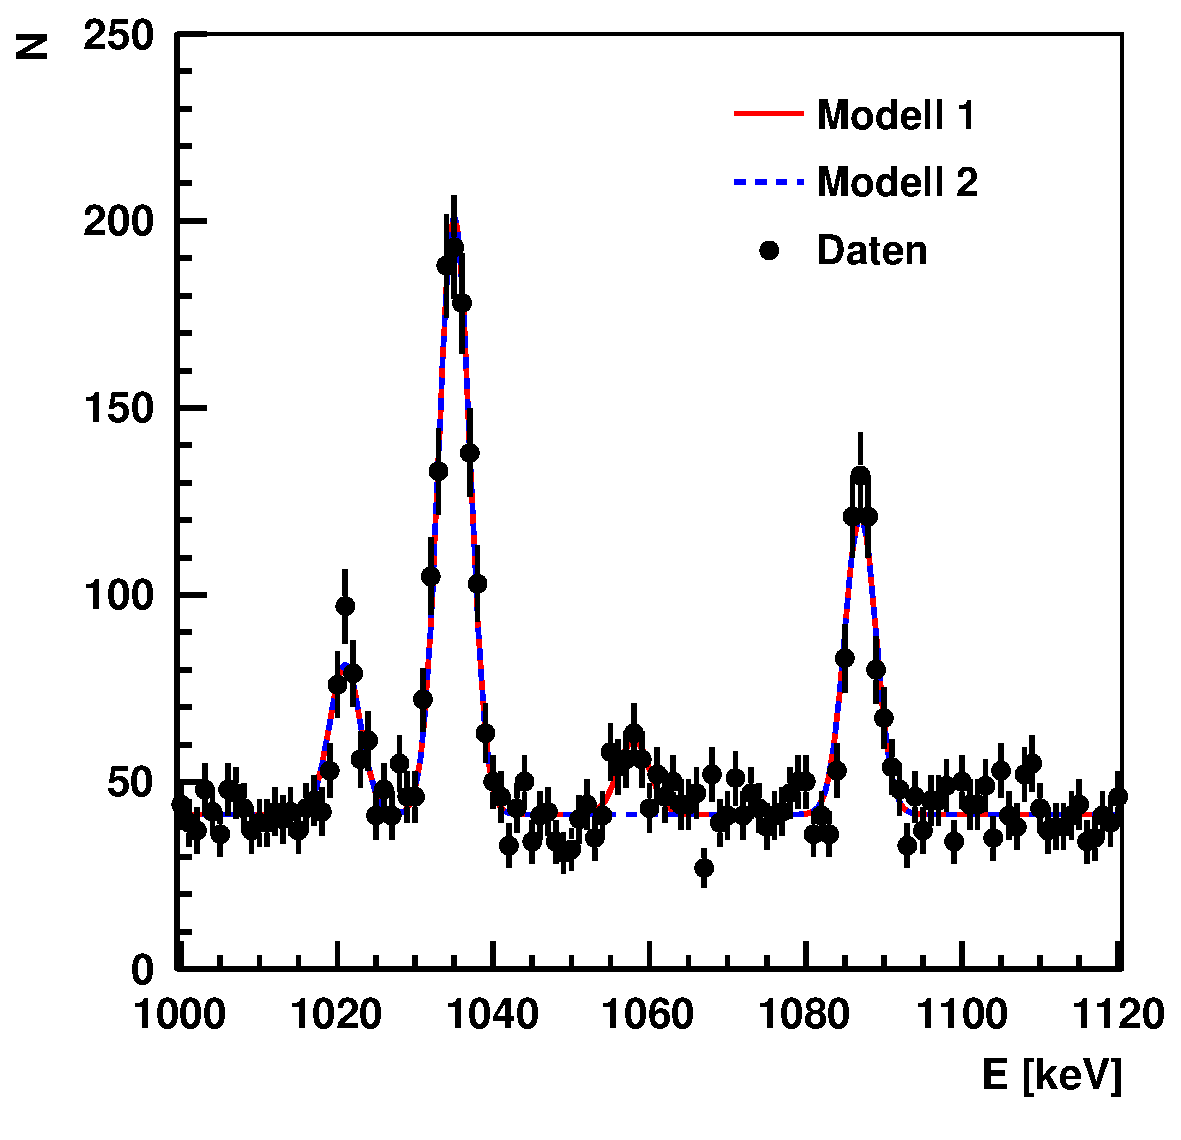
\includegraphics[width=0.5\textwidth]{plot.pdf}
%    \caption{A figure caption~\cite{brandt}.}
%    \label{fig:fig1}
%  \end{center}
%\end{figure}
